%\documentclass[xcolor=dvipsnames]{beamer}
\documentclass[mathserif,10pt]{beamer}

\mode<presentation>
{
  \usetheme{UIUC}
} 

\newcommand{\cmt}[1]{}
\setbeamercovered{transparent=50}
\newcommand{\LIR}{{\tt LLVM IR}}
\newcommand{\MC}{{\tt Machine Code}}
\usepackage{listings}
\usepackage{amsmath}

\title[allvm]{allvm - Binary Decompilation}
\author{Sandeep Dasgupta}
\institute[UIUC]{University of Illinois Urbana Champaign}
\date{\today}


%if u want to show off the sections only
\setcounter{tocdepth}{1}

\lstset{language=[ANSI]C}
\lstset{% general command to set parameter(s)
  basicstyle=\footnotesize\tt, % print whole listing small
    identifierstyle=, % nothing happens
    commentstyle=\color{red}, % white comments
    showstringspaces=false, % no special string spaces
    lineskip=1pt,
    captionpos=b,
    frame=single,
    breaklines=true
      %\insertauthor[width={3cm},center,respectlinebreaks]
}



% If you want to come back to the subsection in outline everytime:
%\AtBeginSubsection
%{
%  \begin{frame}<beamer>{Outline}
%    \tableofcontents[currentsection,currentsubsection]
%  \end{frame}
%}

\AtBeginSection
{
  \begin{frame}<beamer>{Outline}
    \tableofcontents[currentsection,currentsubsection]
  \end{frame}
}


\begin{document}

\begin{frame}
\titlepage
\end{frame}


%%%%%%%%%%%%%%%%%%%%%%%%%%%%%%%%%%%%%%%%%%%%%%%%%%%%%%%%%%%%%%%%%%%%%%%%%%%%%%%%%%%%%
\section{Goal \& Motivation}
\subsection{Research Goal} %3:25 
\frame
{
  \frametitle{\subsecname}
  \begin{itemize}
    \item Research Goal
      \begin{itemize}
        \item Obtain ``richer'' LLVM IR than native machine code.
        \item Enable advanced compiler techniques ( e.g. pointer analysis, information flow tracking, automatic vectorization)
      \end{itemize}
  \end{itemize}

  \cmt{ 
    Today I will be presenting our work on binary dec ... 
      First I will start with the research goal which is to 
      obtain a richer version of llvm IR than the machine code 
      which entails more source level information (like variable , type , aggregate structures,
       control flow,    ) than the native binary

      A related goal is that having such a  rich IR 
      we can do many sophisticated analysis, optimizations and code generation on them
      enable various compiler 
      analysis like pointer analysis, ...

      [Information flow in an information theoretical context is the transfer of information from a variable x to a variable y in a given process.
Not all flows may be desirable. For example, a system should not leak any secret (explicitly or implicitly) to public observers. ]

    /*
       Goal involves experimental understanding of the trade-offs between
      different approaches to reconstructing a richer IR.
      */

    why llvm ir: 
      sophisticated analysis, optimization, and code generation for code from arbitrary languages
             at arbitrary points in the lifetime of software. The diff points could be 
             compile time, link time, install time, load time, run-time,
           “idle-time” 
  }
}

\subsection{Why ``richer'' LLVM IR} 
\frame
{
  \frametitle{\subsecname}
   \begin{itemize}
      \item Source code analysis not possible
        \begin{itemize}
          \item IP-protected software 
          \item Malicious executable 
          \item Legacy executable
        \end{itemize}
      \item Source code analysis not sufficient
        \begin{itemize}
          \item What-you-see-is-not-what-you-execute
        \end{itemize}
  %    \item End-user security enforcement
      \item Platform aware optimizations
    \end{itemize}

  \cmt{ 
  Absence of source-code: There are several scenarios where the original
source-code is not accessible. 
below: 
  - IP-protected software 
  - Third-party library and software components
  - Malicious executable 
  - Legacy executable 

  All such situations analysis of a HLIR is more beneficial than execuatble analyis
  For example, in case of IP protected sf or a known Malicious software, 
  in order to certify the behavior and uncover vulnerabilities HLIR analysis is 
  more benefial than exec analysis because the former contain HL source code semantics.  
    
    Also for legacy executable for which no 
    source code is avalailable aand running on outdated config.... executable 
    analysis is required which can recover functionally correct
      source-code components from such legacy software, so that such legacy
      systems can be ported to secure configurations. 

  even if we have the source code, exectatble analysis after 
  converting it to IR is more beneficial than source code analysis.

  Source-code analysis not sufficient
    There are several scenarios An executable code might demonstrate differ- ent behavior from
    the original source code. This phenomenon is popularly known as
    What-you-see-is-not-what-you-execute 
    Modifications can happen to the source code during compilation
    (optimizations) or after the compilation process (bad code injection).
    These modifications can significantly alter the program behavior. Con-
    sequently, the exact behavior of any program can only be uncovered by
    analyzing the executable code and the analysis of the exec is much more effective if
    done at the hihger level

    /*
       Moreover, several components of a typical software might be developed in
    multiple languages (Fortran, C and C++). 
    The analysis of the source code with diff lang is more diff
    that the analysis of the exec havinga consistent rep.
  */

  End-user security enforcement.: proposal pdf
  The software available to the end user is often in eec format w/o the source code
  and enforcing security features at that level is 
  difficult beciase of the absence of any semantic knowledge about the program,

  so extracting a high level IR is beneficial i this scenario

  Platform aware optimizations
    Binaries compiled for wide distribution are often targeted for one
    particular ISA and are rarely optimized for a particular processor.  Binary
    tools on an end-user platform can apply custom transforma- tions to take
    advantage of platform-specific information like exact knowledge of the
    memory hierarchy or the precise version of multimedia instructions.
  
  }
}

%%%%%%%%%%%%%%%%%%%%%%%%%%%%%%%%%%%%%%%%%%%%%%%%%%%%%%%%%%%%%%%%%%%%%%%%%%%%%%%%%%%%%
\section{Possible Approaches}
  \subsection{The 3 Possible Approaches} % 4:37 (+7.62)
  \frame
  {
    \frametitle{\subsecname}
    \begin{itemize}
      \item Decompile \MC \ $\rightarrow$ \LIR
      \item ``Annotated'' \MC \ $\rightarrow$ \LIR
      \item Ship \LIR
    \end{itemize}


    \cmt{ There are 3 possible approaches to achieve the goal; As u can see all
      of them are having atradeoff between odoption and quality of llvm ir }

  }

  \subsection{Decompile \MC \ $\rightarrow$ \LIR}
  \frame
  {

    \frametitle{\subsecname}
  \begin{table}[]
    \centering
    \label{my-label}
    \begin{tabular}{|p{0.4\textwidth}|p{0.4\textwidth}|}
    \hline
      \multicolumn{1}{|c|}{Benefits} & \multicolumn{1}{|c|}{Challenges} \\ \hline
    \begin{itemize}
      \item Easy to adopt
      \item No compiler support needed
    \end{itemize}  
    &            
    \begin{itemize}
      \item Reconstructing code and control flow
      \item Variable recovery
      \item Function \& ABI rules recovery
    \end{itemize}  
      
      \\ \hline
    \end{tabular}
  \end{table}

  \begin{itemize}
    \item Tools Available: QEMU, BAP, Dagger, Mcsema, Fracture
  \end{itemize}
      



    \cmt{
    \begin{itemize}
      \item Benefit:
        \begin{itemize}
          \item Easy to adopt
          \item No compiler support needed
        \end{itemize}
      \item Challenge: Quality     
      \begin{itemize}
        \item Reconstructing code and control flow - much researched.
        \item Variable recovery
        \item Function \& ABI rules recovery
      \end{itemize}
    \end{itemize}

to <read> .. his is easy to adopt adn mos of the programstoday are shipped as native binaries
  also no extra compiler support is needed

        These methods make various trade-offs between ease of adoption, binary size,
        ease of shipping, and quality of the resulting LLVMIR, which directly
          affects the benefits that allvm provides.

          \item Diffrentiate data \& code.
          \item Indirect branch/call.
          \item Variable instruction size
          \item Position independent code (PIC) sequences
          \item Hand crafted assembly code

    This point is very well researched and exists varisus tools QEMU[8], BAP [7], Dagger [6], and Fracture [23].
    }


  }


  \subsection{``Annotated'' \MC \ $\rightarrow$ \LIR}
  \frame
  {
    \frametitle{\subsecname}

  \begin{table}[]
    \centering
    \label{my-label}
    \begin{tabular}{|p{0.4\textwidth}|p{0.4\textwidth}|}
    \hline
      \multicolumn{1}{|c|}{Benefits} & \multicolumn{1}{|c|}{Challenges} \\ \hline
    \begin{itemize}
      \item Effective  reconstruction
      \item Minimal compiler support needed
    \end{itemize}  
    &            
    \begin{itemize}
      \item Annotations must be
      \begin{itemize}
        \item Minimal   
        \item Compiler \& IR independent
      \end{itemize}
      \item Adoption
    \end{itemize}  
      
      \\ \hline
    \end{tabular}
  \end{table}

  \begin{itemize}
    \item Tools Available: None
  \end{itemize}


\cmt{ 
    \begin{itemize}
      \item Benefit: 
        \begin{itemize}
          \item Effective reconstruction of higher level IR
          \item Minimal compiler support needed
        \end{itemize}
      \item Challenge: 
        \begin{itemize}
          \item Annotations must be ``minimal'' \& sufficient
          \item Annotations must be compiler \& IR-independent
          \item Adoption
        \end{itemize}
    \end{itemize}
  
  
  Seconf is to generate the binaru woth some annotations on it, which help help in
  recpnsruct the hogh kevel ir
  This requires compiler support but the goal here to to genetate minimal annotions
  which is sufficient to generate an high leve ir
  
  Another challenge is that the annotations should be compiler- and
  IR-independent, e.g., a non-LLVM commercial compiler such as Windows Visual
    C++ or Intel’s ICC should be able to produce them 

    what is the minimal information sufficient to reconstruct LLVM IR, so that
    redundant information is not encoded. A third question is how to encode the
    information compactly on native code, so that it does not blow up the size
    of executables.  1.2.3
    
    * Add another bullet
    here saying that we will learn from our experience with the first approach
    before we decide what the annotations need to be
}

  }

  \subsection{Ship \LIR}
  \frame
  {
    \frametitle{\subsecname}
  \begin{table}[]
    \centering
    \label{my-label}
    \begin{tabular}{|p{0.4\textwidth}|p{0.4\textwidth}|}
    \hline
      \multicolumn{1}{|c|}{Benefits} & \multicolumn{1}{|c|}{Challenges} \\ \hline
    \begin{itemize}
      \item \emph{No loss} of information
    \end{itemize}  
    &            
    \begin{itemize}
      \item Adoption in Non LLVM based compilers
      \item Code size bloat
    \end{itemize}  
      
      \\ \hline
    \end{tabular}
  \end{table}

  \begin{itemize}
    \item Tools Available: Portable Native Client, Renderscript, iOS, watchOS and tvOS apps.
  \end{itemize}



\cmt{
    \begin{itemize}
      \item Benefit:
        \begin{itemize}
          \item \emph{No loss} of information via conversion to and from binary code.
        \end{itemize}
      \item Challenge:
        \begin{itemize}
          \item Adoption in Non LLVM based compilers
          \item Stable distribution format for shipping  
          \item Risks to intellectual property
          \item Code size bloat
        \end{itemize}
    \end{itemize}

  Thrisd is to ship ir directly; Obviously there will be no info loss

  There are compilers that do not use LLVM IR as an internal representation.

    The best solution for such compilers would be to treat LLVM IR as a target
    for producing code, 
      Glassgow haskell compiler supprts backend to support llvm 3.5
      such as the Dragonegg plugin that takes code compiled
      by GCC and converts it to LLVM IR instead. 
      
        LLVM IR is a relatively simple, orthogonal instruction set with
        an unlimited number of registers and targeting LLVM IR should be much
        easier than a back end for a native hardware architecture. 
        

        LLVMIR is not a fully frozen and stable ABI
     However, two commercial projects – Portable
     Native Client and Renderscript – are already shipping LLVM IR in modified
     form, so it is not an insurmountable barrier. 
     

     many commercial Java and .NET applications are shipped in rich bytecode
     languages (JVM or MSIL) that reveal extensive source-level semantic
     information. The way they reduce the risk to their intellectual property
     is to use deliberate obfuscation tools, e.g., ProGuard or DexGuard, which
     are far more effective than relying on standard binary code to prevent
     reverse engineering. If such tools can protect applications shipped in
     relatively high-level representations like JVM or MSIL, the techniques
     they use could be applied equally effectively to LLVM bitcode as well.
        
** Note: "Ship LLVM IR with machine code" already exists!  But requires source code and an LLVM-based compiler

http://thenextweb.com/apple/2015/06/17/apples-biggest-developer-news-at-wwdc-that-nobodys-talking-about-bitcode/
IN world wide developer conference 2015, apple mentions how shipping llvm
bytecode optimize the installation of iOS, tvOS, and watchOS apps.  apps can
automatically take advantage of new processor capabilities they might be adding
in the future, without the app developers resubmitting to the store.

  }
}

%%%%%%%%%%%%%%%%%%%%%%%%%%%%%%%%%%%%%%%%%%%%%%%%%%%%%%%%%%%%%%%%%%%%%%%%%%%%%%%%%%%%%%
\section{Our Approach}
  \subsection*{Our Approach}
  \frame
  {
    \frametitle{\subsecname}

    \underline{Long term goal} \vspace{1mm} \\
    Minimal compiler-independent annotations to reconstruct high-quality IR

    \vspace{5mm}
    \underline{Short term goals} \\
        \begin{enumerate}
          \item Experiment with \MC\ $\rightarrow$ \LIR, to \textbf{understand} the challenges better
            \begin{itemize}
              \item To select an existing decompilation framework.
              \item Experiment with different variable and type recovery strategies
            \end{itemize}    
          \item Design suitable annotations for what cannot be inferred without them
        \end{enumerate}    

      \cmt{

** Note: "Ship LLVM IR with machine code" already exists!  But requires source code and an LLVM-based compiler
      }
  }

  \subsection{Selecting mcsema}
  \frame
  {
    \frametitle{\subsecname}
    \begin{itemize}
      \item Actively supported and open sourced
      \item Well documented
      \item Functional \LIR
      \item Separation of modules: CFG recovery and CFG $\rightarrow$ \LIR
    \end{itemize}

    \begin{figure}[h]
      \centering
        \scalebox{0.45}{
          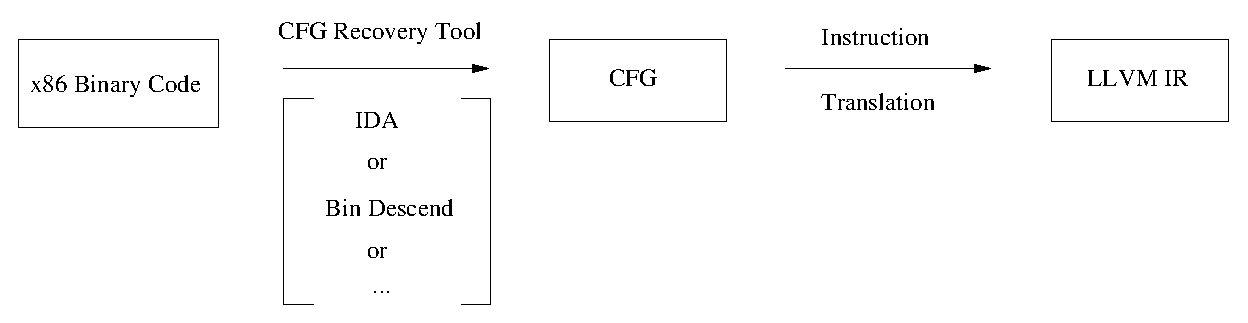
\includegraphics{Figs/3.eps}
        }
    \end{figure}

    \cmt{ 

      we briefly looked at several of the
        existing x86-to-LLVM projects before deciding on mcsema. This decision
        was made largely on the basis that mcsema is the most well-maintained
        and furthest along of the other projects.
    
      The translator is broken into two components: control flow recovery and
      translation. These components are two separate applications and can operate
        independently of each other. 
        
        Following is a typical usage diagram of  the tool:
        In typical usage, a program's control flow
        graph (CFG) is recovered and then the CFG is immediately transcribed into
        LLVM. 


    Control Flow Recovery:

    Control flow recovery is performed by a recursive descent work list driven
    algorithm that starts from an entry point and decodes blocks and functions. New
    function entry points are identified from branch, jump, and call instructions,
             and from relocations in the original program. 
               
    Control flow recovery is the risky part of translation, because some elements
    are difficult to determine statically. For example, certain kinds of indirect
    branches that are not supported in this initial release. To determine the
    target of a branch such as jmp <reg32> would require either outside input from
    traces, or, some kind of iterative data flow analysis. While an interative
    analysis would be possible in this framework, it is not currently supported.

    }
  }



  \subsection{Instruction Translation: Memory Model}
  \frame
  {
    \frametitle{\subsecname}

    \begin{figure}[h]
      \centering
        \scalebox{0.45}{
          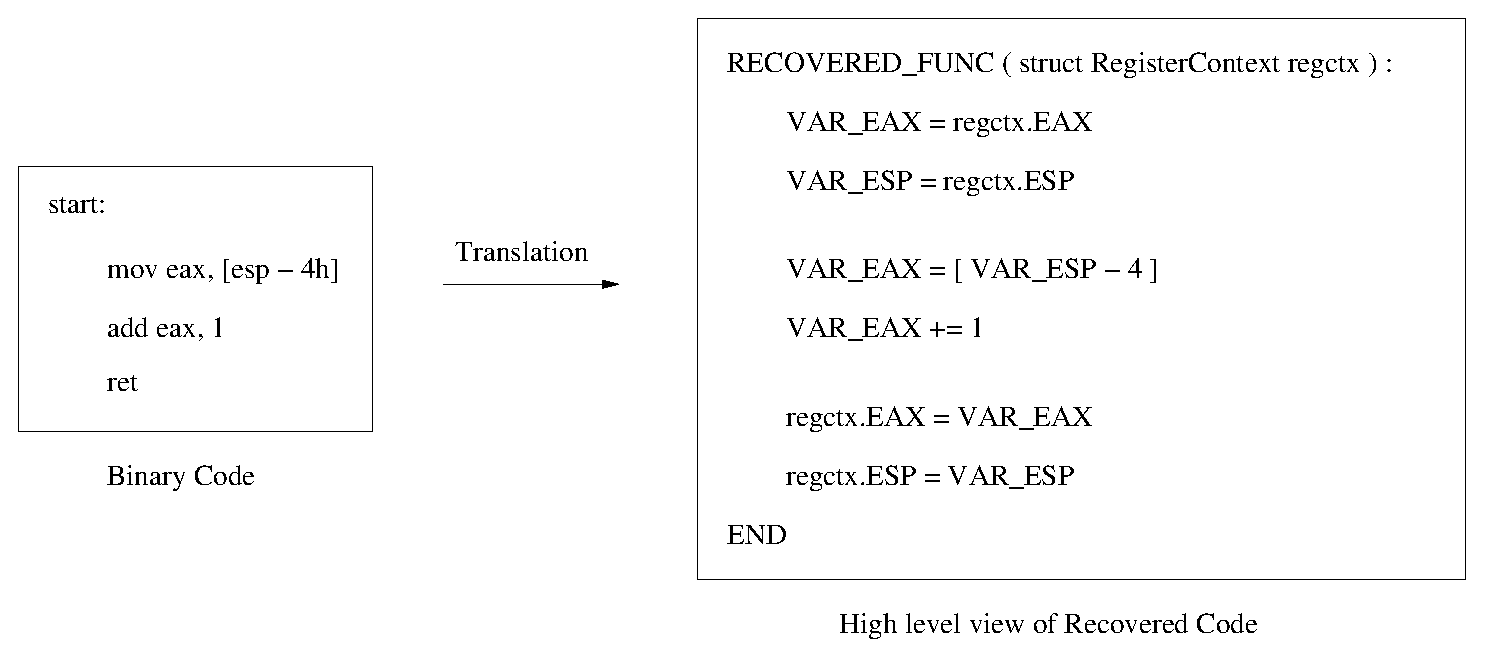
\includegraphics{Figs/4.eps}
        }
    \end{figure}
      
    \cmt{
    Instruction Translation

    Each function is given, as input, a structure that represents the current
    register context. 
    Every general-purpose register (GPR) on the supported platform is represented
    as a local variable of an integer type of the appropriate bit-width.
    
    Each function then has a prologue that will copy from the
    input state to local state. 
    
    Every time control would transfer out of the
    function, local state is written back into the state structure and then either
    passed to return, or passed to child functions.



    Sub-registers (such as ax, bx, cx, dx, ah, al, etc) are not represented by
    their own variables. When a sub-register is read or written, bit-shifting
    operations are produced that will read or write the selected bits from each
    local variable.

    }

  }

  \subsection{mcsema: Demo}
  \frame
  {
    \frametitle{\subsecname}
    \cmt{
    The inspiration behind representing registers as LLVM local variables is the
    memory to register transformation pass in LLVM. This pass can take code that
    has variables, in the form of locally allocated memory cells that are loaded
    from and stored to, and promotes those variables into SSA values. Once the code
    is in SSA form, common optimizations like merging, constant folding, and dead
    code elimination, can be used on the translated code.

    These optimizations are beneficial to the translator because translating
    semantics is very noisy. To accurately represent each instruction, all of its
    side-effects must be represented as well. Many side effects are dead on
    arrival, commonly flag writes which are dominated by another flag write. It
    would be prohibitive for a translator to also maintain flow-sensitivity while
    translating, so instead, we have a very noisy first pass that emits every
    possible side effect and then use a standard compiler optimization to remove
    dead or meaningless side effects.

    This has a few advantages and disadvantages. The chief disadvantage is that
    this does not represent stack-passed parameters in the LLVM. However, this
    information is lost during compilation from source language to native
    instructions and is only available by recovery and analysis of memory loads
    relative to the stack / base pointer. Since all of the semantics are captured
    by translation, it is conceivable that an analysis pass can consume the LLVM
    bitcode, discern parameter slots on the stack, and promote those into arguments
    that are passed to the function.

    An advantage, related to parameter passing, is that this representation is
    capable of capturing parameter-passing schemes that use registers. Callers can
    use those schemes by simply writing the parameters into the appropriate
    register structure before calling the child function.
    }

  }

  \subsection{Support \& Limitations}
  \frame
  {
    \frametitle{\subsecname}
    \begin{itemize}
      \item What Works
        \begin{itemize}
          \item Integer Instructions
          \item FPU and SSE registers
          \item Callbacks, External Call, Jump tables 
        \end{itemize}
      \item In Progress
        \begin{itemize}
          \item FPU and SSE Instructions: Not fully supported
          \item Exceptions
          \item Better Optimizations
        \end{itemize}
    \end{itemize}
  }

\section{Ongoing Work}
  \subsection{Variable \& Function Parameter Recovery}
  \frame
  {
    \frametitle{\subsecname}
    \begin{itemize}
      \item Benefit
        \begin{itemize}
          \item Enables many fundamental analysis (Dependence, Pointer analysis)
          \item Functional IR
        \end{itemize}
      \item State of the art
        \begin{itemize}
          \item Divine
            \begin{itemize}
              \item State of the art variable recovery %Not scalable 
            \end{itemize}     
          \item Second Write 
            \begin{itemize}
              \item Heuristics for function parameter  detection
              \item Scalable variable and type recovery
            \end{itemize}     
          \item TIE %(Type Inference On Execuatbles)
            \begin{itemize}
              \item Type recovery
            \end{itemize}     
        \end{itemize}
    \end{itemize}

    \cmt{
      Not scalable
    }

  }





\section*{Backup} 
  \subsection{What-you-see-is-not-what-you-execute} 
  \frame
  {
    \frametitle{\subsecname} 
    The following compiler (Microsoft C++ .NET) induced vulnerability was discovered
               during the Windows security push in 2002
    \begin{figure}[h]
      \centering
        \scalebox{0.75}{
          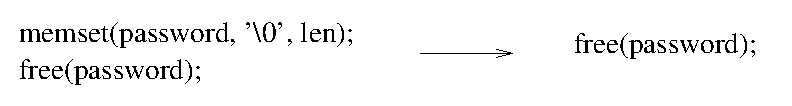
\includegraphics{Figs/2.eps}
        }
    \end{figure}
    \cmt{
               fragment shown in the following on the left never uses the
               values written by memset (intended to scrub the buffer pointed
                  to by password), the memset call could be removed, thereby
              leaving sensitive information exposed in the freelist at
              runtime.  
              
              memset(password, �\0�, len); free(password); =�
              free(password); 

     For instance, in C and C++ the order in which actual parameters are eval-
       uated is not specified: actuals may be evaluated left-to-right,
             right-to-left, or in some other order; a compiler could even use
               different evaluation orders for different functions. Different
               evaluation orders can give rise to different be- haviors when
               actual parameters are expressions that contain side effects. For
               a source-level analysis to be sound, at each call site it must
               take the join (?) of the results from analyzing each permutation
               of the actuals.3 In contrast, an analysis of an executable only
               needs to analyze the particular sequence of instructions that
               lead up to the call

    }
  }




















\end{document}


